\section{Discussion}
As neighbour product selection (Task 1) is an unsupervised approach whose ultimate goal is to support product summarization (Task 2),  I only report the experimental results on Task 2 to demonstrate my model's superiority over the baselines across different timestamps. The efficacy of each input component is also presented here.

\subsection{Automatic Evaluation}

I run my model ten times and report the average evaluation results in the left part of Table \ref{tab:auto-eval}. To verify my model's superiority, I calculate the performance differences between my model and each baseline on each automatic metric for all the ten runs, and apply a t-test on the ten differences to check whether the performance difference is significant. 

RT performs the worst as the product title contains limited and static information to reveal product sentiment dynamics. From TR results, adding sparse reviews can improve model performance, but is still worse than the rest approaches, which strongly indicates the effectiveness of using neighbour product reviews for generating aspect summarization. Most of neighbour selection based baselines have roughly similar results except TS model, meaning that behavior based is better than content based neighbour selection. Surprisingly, Random model can achieve a relatively satisfying result. One possible reason is that because most of reviews in online shopping websites are positive, randomly sampled neighbour product might receive reviews containing relevant sentimental phrases. Howsoever, my BDS model outperforms all baselines significantly (\textit{p$<$0.01}) on all metrics, demonstrating the superiority of my proposed reinforcement neighbour selection.
 

\begin{table}
	% \scriptsize
	
%	\small
	\centering
%	\renewcommand{\tabcolsep}{3pt}
	
	\begin{tabular}{ccccccc} 
		\toprule
		\multirow{2}{*}{ \textbf{Model}}&  \multicolumn{4}{c}{\textbf{Automatic}} & \multicolumn{2}{c}{\textbf{Human }}\\ \cmidrule(lr){2-7}
		&RG-1&RG-2&RG-L&METEOR &WTR &WCR \\ \midrule 
		RT &  36.19 & 10.01 & 27.95 & 16.05& 0.00&0.01\\ 
		TR& 43.05  & 19.08 &  33.10  & 19.24 & 0.07&0.13 \\ 
		TS & 42.97  & 18.85  & 32.85  & 19.34 &0.13 &0.24 \\ 
		Random& 44.21 &  19.58 &  33.98  &  19.86 &0.03 &0.13\\ 
		PMF & 45.72 &  20.25  &  35.21  & 20.80 &0.14 & 0.28\\ 
		GBPR& 45.09 &  19.67  &  34.55&  20.36 & 0.32&0.39\\ 
		EALS& 44.66  & 19.50  &  34.28 &    20.32&0.08 &0.17\\ 
		BDS& \textbf{51.11*} & \textbf{23.55*}& \textbf{39.86*} &  \textbf{22.99* }&  \textbf{0.89 }& \textbf{0.81 }\\ \bottomrule
	\end{tabular}
	% \vspace{-0.5em} 
	\caption{Automatic \& human evaluation results of my model compared with baselines. Symbol ‘*’ highlights the cases where my model significantly beats all baselines with $p$ value smaller than 0.01.}
	\label{tab:auto-eval}
	% \vspace{-1em} 
\end{table} 
 
\subsection{Human Evaluation}
The right part of Table \ref{tab:auto-eval} reports the human evaluation result for all the models. Higher WTR and WCR scores indicate the related model can generate better structured summaries from human perspective. For each baseline, WTR and WCR scores are the pairwise comparison results with the BDS model. RT model performs the worst.  And content based methods (RT and TR) also perform worse than neighbour selection based methods in general. GBPR performs much better than the rest baselines. It beats my model in roughly 30\% of summary pairs.  The reported two scores of my model are the average of pairwise comparison results with all baselines, which shows that my model can beat other baselines on 90\% of all summary pairs.

Both automatic and human evaluation results demonstrate content based baselines perform worse than neighbour selection based baselines. However, there are still some inconsistencies between their evaluation results. Although GBPR has similar performance with the rest of neighbour based baselines on automatic metrics, it unexpectedly outperforms on human metrics, which indicates how to organize sequences has huge impact on summary semantic quality.

\subsection{Dynamic Performance} 
\begin{figure} 
	\centering 
	\subfloat[ROUGE-1]{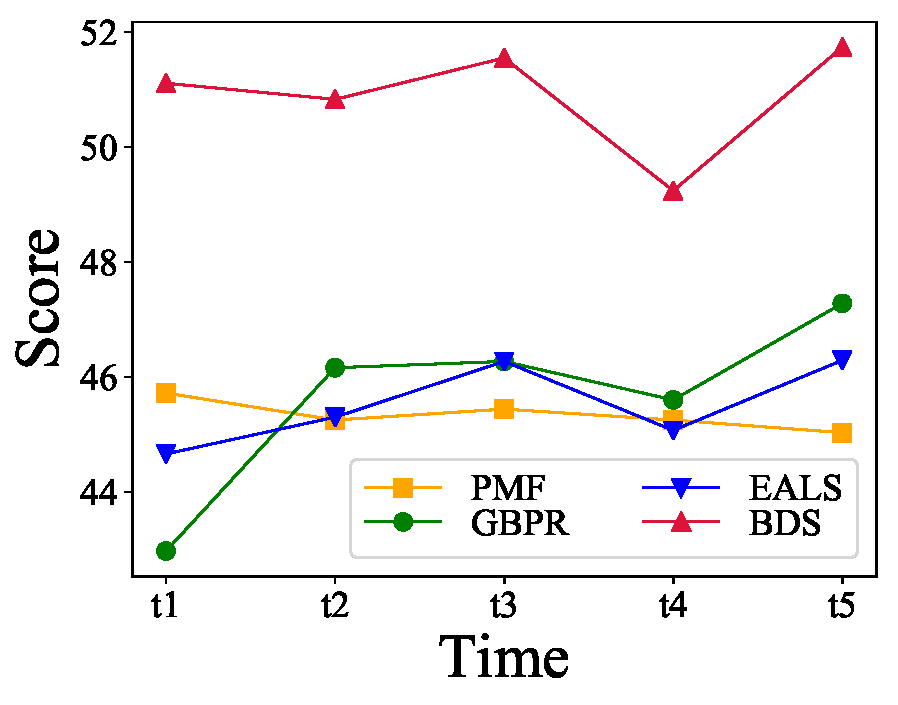
\includegraphics[width = 0.5\columnwidth]{img/chapter5/rouge-1.pdf}}
	\subfloat[ROUGE-2]{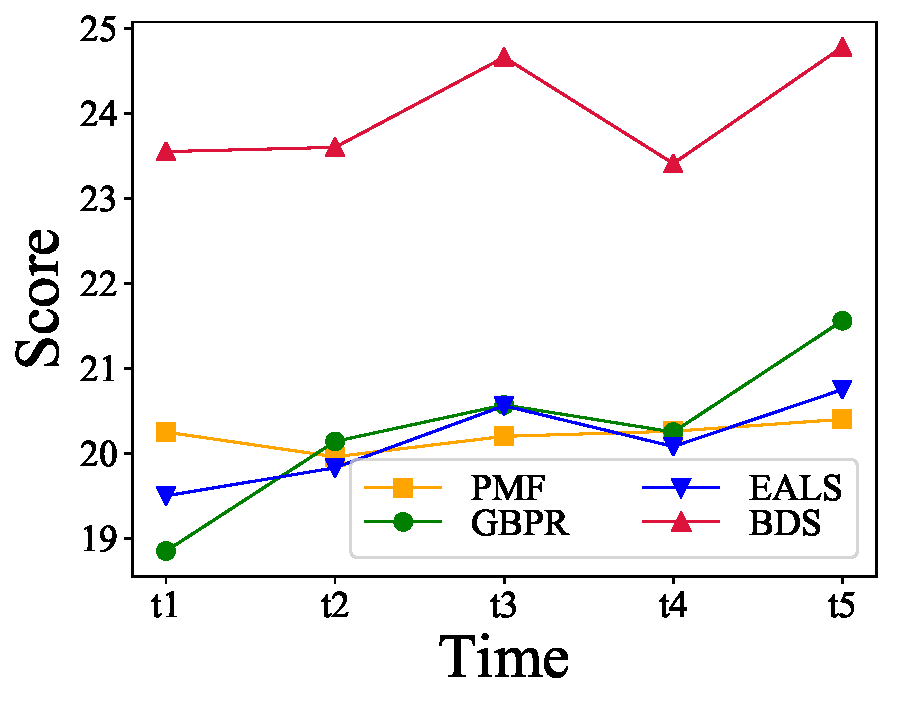
\includegraphics[width =0.5\columnwidth]{img/chapter5/rouge-2.pdf}}\\ 
	\subfloat[ROUGE-L]{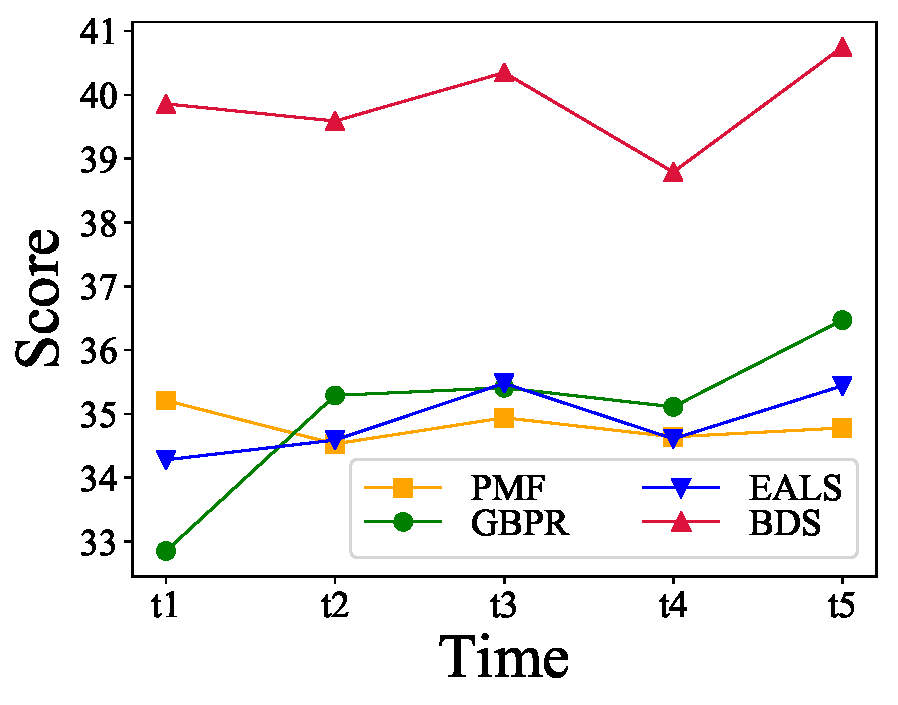
\includegraphics[width = 0.5\columnwidth]{img/chapter5/rouge-L.pdf}}
	\subfloat[METEOR]{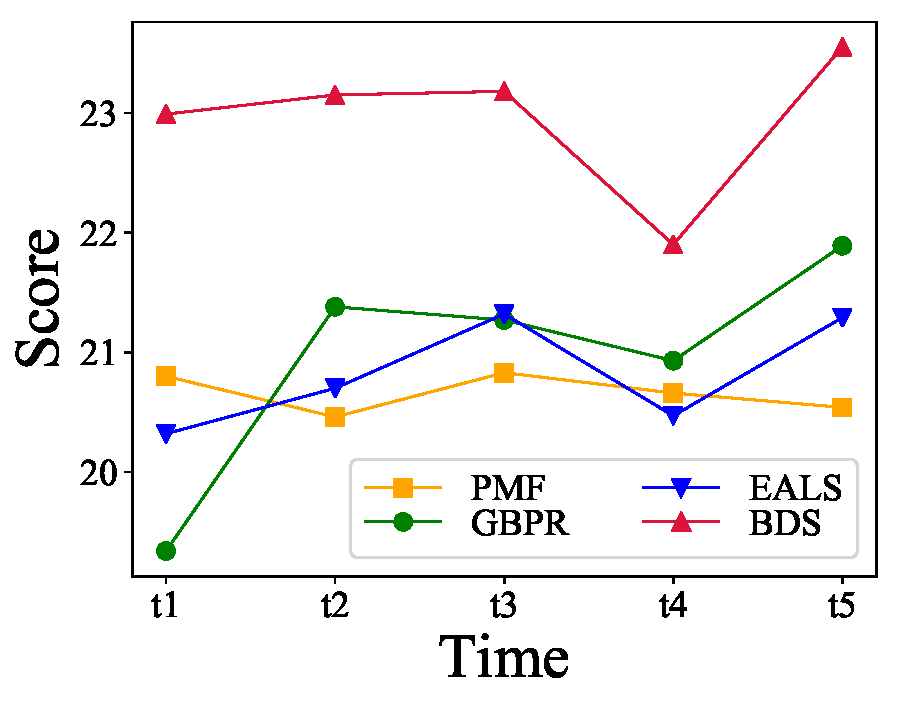
\includegraphics[width = 0.5\columnwidth]{img/chapter5/meteor.pdf}} 
	\caption{Automatic evaluation results of my model compared with the Top 3 baselines in five consecutive time periods ($t_1 \sim t_5$).} 
	\label{fig:auto-eval} 
\end{figure}
To better present my model dynamic performance, I visualize the automatic evaluation results of my model as well as  the best three baselines (PMF, EALS and GBPR) in all five consecutive time periods, shown in Figure \ref{fig:auto-eval}. The three best baselines are all neighbour selection approaches. Across all time periods, all four model performances are relatively consistent and follow similar trend. Their performances go down a little bit in the fourth time period but raise up immediately in the next time period. Among three baselines, GBPR achieves the best performance result over the rest two. It does not perform well in the beginning, but keeps growing and beats the rest baselines in later time periods. In general, the performances of three baselines are not far away from each other, especially from time period $t_2$ to $t_4$. Shown in Figure \ref{fig:auto-eval}, their plotted lines are basically mingled together. However, my model achieves a far better evaluation result than baselines. Its plotted lines (red lines) are always significantly above the rest three lines in terms of all four evaluation metrics. Moreover, model performances on the four reported metrics are with similar trend. And the three ROUGE based metrics are with an even more similar trend than METEOR. 




\subsection{Input Component Evaluation}


As aforementioned, my model requires three types of product input information: user behavior, product category, and profile descriptive phrases. To examine whether all involved information are effective, I conduct an extensive study by removing each type of information iteratively while holding the rest information fixed. Table \ref{tab:ablation} shows the performance difference between the models with truncated input and original BDS model. In detail, removing user behavior (product category) means that only product category (user behavior) is used for sentiment prediction pretraining. Removing product profiles means that only neighbour product sentimental phrases contribute to summarization generation. 
 
\begin{table}%[h]
	% \scriptsize
%	\small
	\centering
%	\renewcommand{\tabcolsep}{7pt}
	\begin{tabular}{ccccc} 
		\toprule
		
		\textbf{Model}& \textbf{RG-1} & \textbf{RG-2} & \textbf{RG-L} & \textbf{METEOR}\\ \midrule  
		-- Behavior &-14.21 & -12.63&-11.37  & -5.72\\  
		-- Category&-4.74 & -2.94&-4.27 & -1.65 \\
		-- Profile &-5.78 & -3.77&-5.33& -2.34\\  
		\bottomrule
	\end{tabular} 
	\caption{Performance differences between the model with truncated input and original BDS model. `--' means removing related input component from my model.}
	\label{tab:c5_ablation} 
\end{table}
From Table \ref{tab:c5_ablation}, removing related input component always leads a decrease on model performance, which indicates that all the three types of input component are useful in BDS model. Compared with product category and descriptive phrases, user behavior obviously has the most influential impact because removing it causes the largest drop in model performance over all four reported metrics. Surprisingly, it declines the model performance down close to the worst baseline, RT. It explicitly verifies the importance of user behavior for product summarization generation. Moreover, the performance decrease by removing profile descriptive phrases is larger than removing product category embedding. The reason might be that profile descriptive phrases are directly used for summarization generation. While product category contributes to the sentiment prediction pretraining, which only has implicit impact and is not able to directly reflect dynamic aspect sentiment changes. 
 
\subsection{Case Study} 
\begin{table}%[h]
%	\scriptsize
	% \small
	\centering
%	\renewcommand{\tabcolsep}{3pt} 
%	\renewcommand\arraystretch{0}
	
	
	\begin{tabular}{p{1cm}p{6cm}p{6cm}} 
		\toprule
		
		\textbf{Time} & \multicolumn{1}{c}{\textbf{Ground Truth}} & \multicolumn{1}{c}{\textbf{BDS}}\\ \midrule 
		$t_1$ & \colorbox{YellowGreen}{\textbf{Material : Positive}} \newline \textbf{Summarization:} The \textcolor{YellowGreen}{\textbf{material}} of the dress is super \textcolor{YellowGreen}{\textbf{nice}} and  \textcolor{YellowGreen}{\textbf{soft to wear}}. It is made of cotton and touches like a   \textcolor{YellowGreen}{\textbf{high-end}} dress. A perfect gift for aged women. & \colorbox{YellowGreen}{\textbf{Material : Positive }} \newline \textbf{Summarization:} The dress has \textcolor{YellowGreen}{\textbf{good material }}. It is made of \textcolor{YellowGreen}{\textbf{cotton and touches very soft}}. A perfect gift for mums who have \textcolor{YellowGreen}{\textbf{high-standard}} requirement on dress material.\\ \midrule 
		$t_2$ & \colorbox{red}{\textbf{Material : Negative }} \newline \textbf{Summarization:} The dress \textcolor{red}{\textbf{material}} is \textcolor{red}{\textbf{not as good as promised}}. It is \textcolor{red}{\textbf{not good}} for aged women with high requirements. It touches as \textcolor{red}{\textbf{cheap material}} and smells weird. & \colorbox{red}{\textbf{Material : Negative }} \newline \textbf{Summarization:} The \textcolor{red}{\textbf{material is terrible}}. It touches like \textcolor{red}{\textbf{carded yarn with much cheaper material}} as promised for mums. It has a weird smell when wearing it. \\ \bottomrule
	\end{tabular}   
	\caption{A real case to show my model's generated dynamic sentiment summarization for a dress on product material. The \textcolor{YellowGreen}{green} color indicates positive words. While \textcolor{red}{red} color indicates negative words.}
	
	\label{tab:c5_demo} 
\end{table} 
We conduct a case study in Table \ref{tab:c5_demo} on an actual dress to show how my model summarize its aspect-sentiment changes in a timely manner. In this case, I only care about sentiment changes on product material and demonstrate material-related content from the full generated summaries. In the real world, the sentiment of the dress material goes from positive to negative (concluded from summarization) due to its manufacturer's counterfeit (reported by customers in time $t_2$). My model is able to  detect this aspect-sentiment change from its updated customer shopping behaviors and dynamically locate neighbour products with similar issues (like material problems). From the result shown in Table \ref{tab:c5_demo}, the generated summaries on `Material' aspect supports my model effectiveness. Moreover, the generated summaries solely contain objective descriptions instead of emotional expressions used in personal reviews, which shows a  more formal and aspect-concentrated way of description than summarized reviews. 
